\section{Исследовательский раздел} \label{research}

\subsection{Цель исследования}

Целью исследования является оценка зависимости времени выполнения запроса от наличия индексов в базе данных. Для оценки использован запрос на языке sql\cite{sql} из листинга \ref{lst:exec_time}. Необходимо определеить влияет ли использование стандартного b-tree индекса на user{\_}id  на время выполнения данного запроса при различном количестве записей.

\begin{lstlisting}[label=lst:exec_time, caption=Запрос для исследования]
select yandex_id, token, login, name, phone, role
from service.users
where login = {login}
\end{lstlisting}

\subsection{Описание исследования}

На первом этапе исследования производится замер времени выполнения запросов при количестве записей от 1000 до 100 000 с шагом 1000 в таблице users без использовния индекса на login.

На втором этапе исследования производится замер времени выполнения запросов при том же количестве записей, что и на предыдущем этапе, однако с использованием индексов.

Для уменьшения погрешности вычислений каждый запрос отправляется 100 раз, а за результат берется медианное время 100 запросов.

Для уменьшения временных издержек, связанных с работой сети база данных и скрипт отправки запросов звпускаются на одной физической машине.

Результаты измерений приведены в таблице \ref{tab:measure}. График изображен на рисунке \ref{fig:graph}.

\pagebreak

\begin{table}[ht!]
	\centering
	\caption{Результат исследования}
	\label{tab:measure}
	\begin{tabular}{|p{5.5cm}|p{4cm}|p{4cm}|}
		\hline
		\textbf{Количество записей} & \textbf{С индексом, с} & \textbf{Без индекса, с} \\
		\hline
		5000 & 0.001 & 0.001 \\
		\hline
		10000 & 0.001 & 0.001 \\
		\hline
		15000 & 0.0 & 0.001 \\
		\hline
		20000 & 0.002 & 0.002 \\
		\hline
		25000 & 0.002 & 0.002 \\
		\hline
		30000 & 0.003 & 0.004 \\
		\hline
		35000 & 0.004 & 0.005 \\
		\hline
		40000 & 0.006 & 0.005 \\
		\hline
		45000 & 0.007 & 0.007 \\
		\hline
		50000 & 0.008 & 0.008 \\
		\hline
		55000 & 0.01 & 0.01 \\
		\hline
		60000 & 0.011 & 0.011 \\
		\hline
		65000 & 0.013 & 0.016 \\
		\hline
		70000 & 0.014 & 0.018 \\
		\hline
		75000 & 0.015 & 0.02 \\
		\hline
		80000 & 0.017 & 0.027 \\
		\hline
		85000 & 0.02 & 0.032 \\
		\hline
		90000 & 0.021 & 0.037 \\
		\hline
		95000 & 0.022 & 0.038 \\
		\hline
	\end{tabular}
\end{table}

\begin{figure}[h!]
	\centering{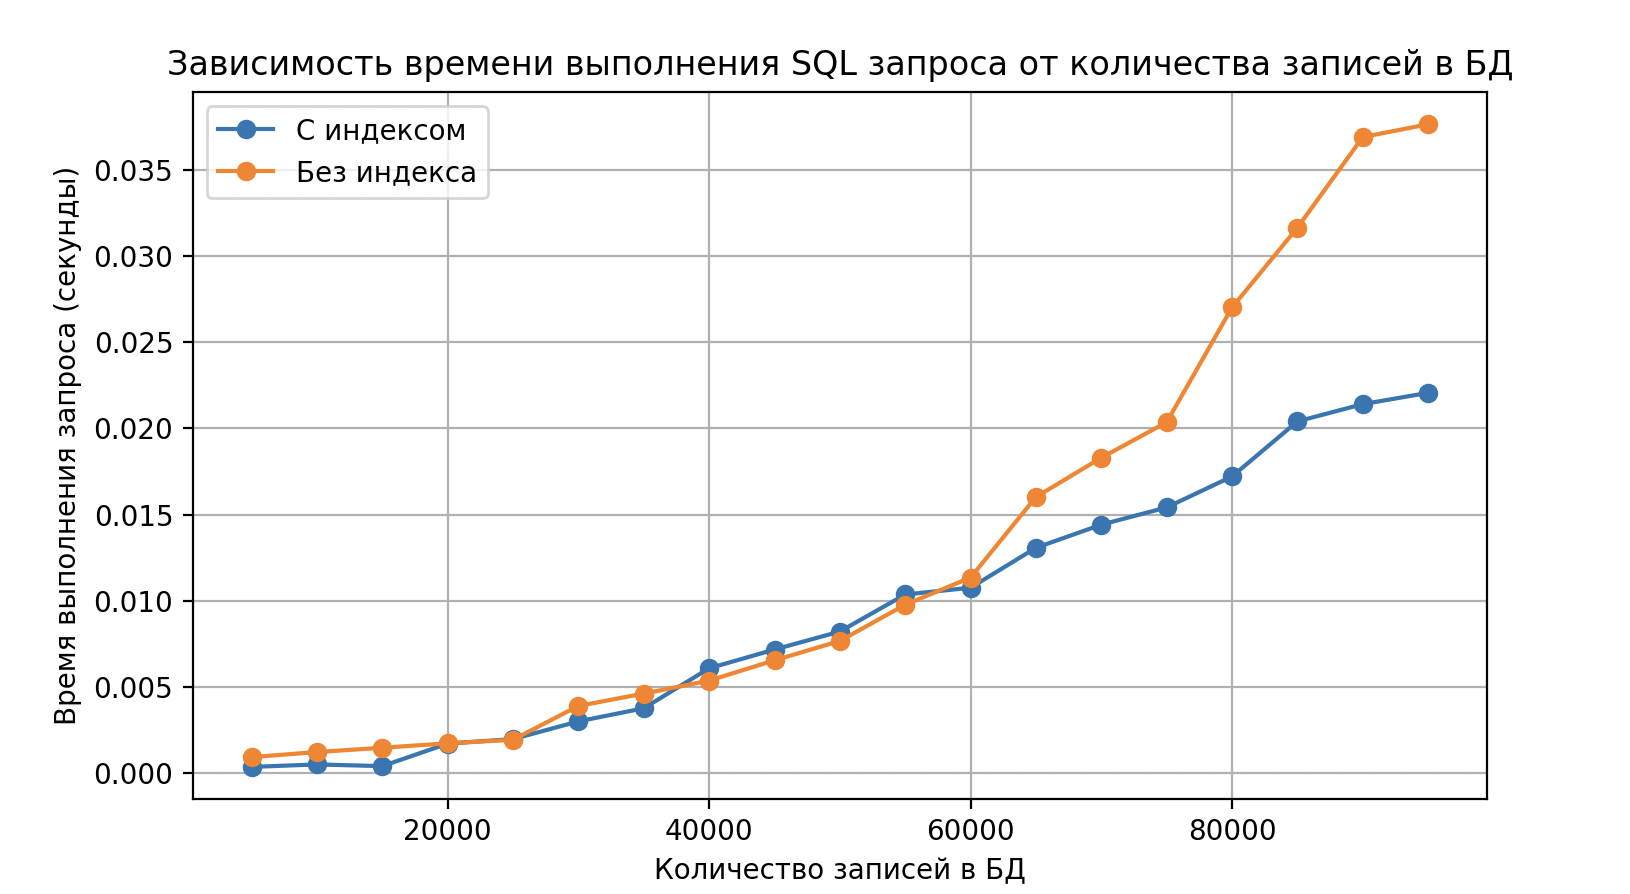
\includegraphics[scale=0.55]{img/graph.png}}
	\caption{График измерений}
	\label{fig:graph}
\end{figure}

\subsection{Вывод}

В результате исследования установлено, что для запроса из листинга \ref{lst:exec_time} время выполнения уменьшается при использовании индексов после определенного порогого числа записей (60 000 в данном исследовании). При меньшем количестве записей использование индексов не дает особого преимущества во времени выполнения запроса.

\pagebreak